\documentclass[10pt,a4paper]{article}
\usepackage[margin=1.2cm]{geometry}
\usepackage{booktabs,array,xcolor,multicol,tikz,enumitem,parskip}
\usetikzlibrary{shapes.geometric,arrows.meta,positioning,fit,backgrounds}
\setlength{\parindent}{0pt}
\setlength{\parskip}{2pt}
\setlength{\columnsep}{0.8cm}

\definecolor{navy}{RGB}{15,35,64}
\definecolor{teal}{RGB}{0,150,136}
\definecolor{green}{RGB}{27,135,59}
\definecolor{red}{RGB}{198,40,40}
\definecolor{amber}{RGB}{230,92,0}
\definecolor{lgrey}{RGB}{240,244,248}
\definecolor{blue}{RGB}{26,74,138}

\newcommand{\hd}[1]{\medskip\textcolor{navy}{\textbf{\large #1}}\par\noindent\rule{\linewidth}{0.6pt}\smallskip}
\newcommand{\badge}[2]{\colorbox{#1}{\textcolor{white}{\footnotesize\textbf{#2}}}}

\begin{document}
\pagestyle{empty}

% ── HEADER ────────────────────────────────────────────────────────────────
\colorbox{navy}{\parbox{\linewidth}{\vspace{4pt}\centering
  \textcolor{white}{\LARGE\textbf{LecSeg-30}} \quad
  \textcolor{cyan!60!white}{\large A Reproducible Low-Resource Benchmark \& Diagnostic Study}\\[2pt]
  \textcolor{white!70!navy}{\normalsize Lecture-Video Topic Segmentation \quad|\quad Supervisor Reference Sheet}
\vspace{4pt}}}

\medskip
\begin{multicols}{2}

% ── LEFT COLUMN ───────────────────────────────────────────────────────────
\hd{The Problem}
Students cannot navigate 3-hour lecture recordings without chapter markers.
\textbf{Goal:} automatically partition a lecture transcript into coherent topic segments.
\textbf{Reference:} YouTube creator-supplied chapter timestamps (navigation metadata, not pedagogical gold standard).

\medskip
\colorbox{lgrey}{\parbox{\linewidth}{\small
\textbf{Three notions of ``topic boundary'' (key conceptual distinction):}\\[2pt]
\textcolor{amber}{\textbf{1 Discourse}} — rhetorical shift (definition→example). Detected by prosody, discourse markers. \textit{Fine-grained.}\\
\textcolor{blue}{\textbf{2 Semantic}} — embedding-space discontinuity. Detected by sentence transformers. \textit{Medium-grained.}\\
\textcolor{green}{\textbf{3 Editorial}} — creator-placed chapter divider. LecSeg benchmark uses this. \textit{Coarse-grained.}\\[2pt]
Conflating levels 1 and 3 explains every acoustic signal failure.
}}

\hd{Dataset — LecSeg-30}
\begin{tabular}{@{}ll@{}}
30 videos & 5 domains (Bio, CS, Math, Phil, Phys) \\
32.52 h   & total transcribed audio \\
46{,}525  & sentences (spaCy) \\
419       & YouTube chapter boundaries \\
904       & reviewed subtopic labels \\
$\kappa_\text{chapter}=0.535$ & (inflated: both annotators see same YouTube metadata) \\
$\kappa_\text{subtopic}=0.426$ & (genuine human IAA, moderate agreement) \\
\end{tabular}

\hd{Pipeline (end-to-end)}

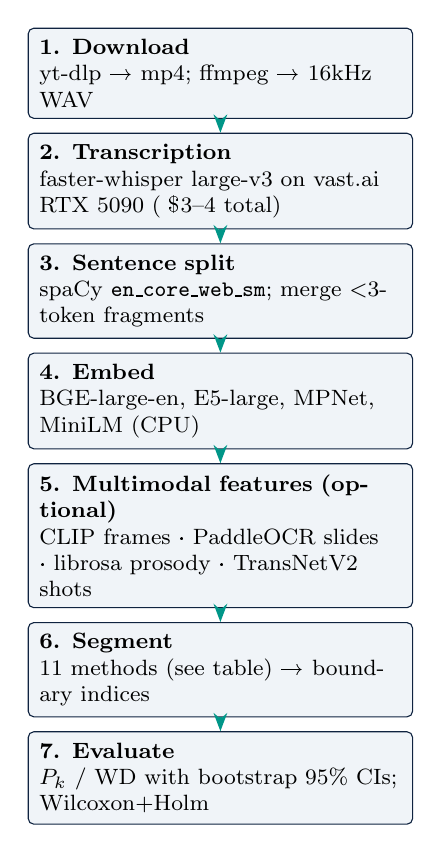
\begin{tikzpicture}[
  box/.style={draw=navy,fill=lgrey,rounded corners=2pt,font=\footnotesize,
              inner sep=4pt,text width=4.6cm,align=left},
  arr/.style={-Stealth,thick,color=teal},
  every node/.style={font=\footnotesize}
]
\node[box] (dl) {\textbf{1. Download}\\ yt-dlp → mp4; ffmpeg → 16kHz WAV};
\node[box,below=5pt of dl] (tr) {\textbf{2. Transcription}\\ faster-whisper large-v3 on vast.ai RTX~5090 (~\$3--4 total)};
\node[box,below=5pt of tr] (sp) {\textbf{3. Sentence split}\\ spaCy \texttt{en\_core\_web\_sm}; merge $<$3-token fragments};
\node[box,below=5pt of sp] (em) {\textbf{4. Embed}\\ BGE-large-en, E5-large, MPNet, MiniLM (CPU)};
\node[box,below=5pt of em] (mm) {\textbf{5. Multimodal features (optional)}\\ CLIP frames · PaddleOCR slides · librosa prosody · TransNetV2 shots};
\node[box,below=5pt of mm] (sg) {\textbf{6. Segment}\\ 11 methods (see table) → boundary indices};
\node[box,below=5pt of sg] (ev) {\textbf{7. Evaluate}\\ $P_k$ / WD with bootstrap 95\% CIs; Wilcoxon+Holm};
\draw[arr] (dl)--(tr); \draw[arr] (tr)--(sp); \draw[arr] (sp)--(em);
\draw[arr] (em)--(mm); \draw[arr] (mm)--(sg); \draw[arr] (sg)--(ev);
\end{tikzpicture}

\columnbreak
% ── RIGHT COLUMN ──────────────────────────────────────────────────────────

\hd{Metrics}
\textbf{$P_k$ (Beeferman 1999)} and \textbf{WindowDiff (Pevzner 2002)} — window-based, lower = better.
Slide a window of width $k = \lfloor N/2K \rfloor$ and count disagreements.
Near-miss boundaries are not fully penalised — appropriate for the navigation task.
$P_k=0.5$ = random; $P_k=0.0$ = perfect.
F1/BS are secondary diagnostics only.

\hd{Methods Tested \& Results}
{\small
\begin{tabular}{@{}lll@{}}
\toprule
Method & $P_k\downarrow$ & Verdict \\
\midrule
TextTiling, KMeansSeg & 0.605, 0.617 & \textcolor{red}{\textbf{Fail}} \\
CosineSeg, BertSeg   & 0.489--0.490 & \textcolor{red}{\textbf{Weak}} \\
C99                  & 0.422        & \textcolor{red}{\textbf{Weak}} \\
BGE-Divisive (baseline) & 0.388     & \textcolor{teal}{\textbf{Best baseline}} \\
CLIP+Text fusion     & 0.374        & \textcolor{green}{\textbf{Good}} \\
Cross-model (E5+BGE) & 0.371        & \textcolor{green}{\textbf{Best $P_k$/WD}} \\
Balanced Selector    & \textbf{0.359} & \textcolor{green}{\textbf{Best mean}} \\
\bottomrule
\end{tabular}}

\hd{Four Pipeline Components (N1--N4)}
{\small
\begin{tabular}{@{}lp{5.5cm}@{}}
\toprule
Label & What it does \\
\midrule
\textbf{N1} & Two-stage predictor: broad pass (high recall) → refinement (high precision) \\
\textbf{N2}$^\star$ & Entropy-weighted fusion: $w(m)\propto e^{-H(m)}$; high-entropy (flat) signals auto-down-weighted \\
\textbf{N3} & Hierarchical enforcer: $\mathcal{B}_\text{chapter}\subseteq\mathcal{B}_\text{subtopic}$ \\
\textbf{N4} & Llama-3.1-8B titling (local, offline); boundary shifting does not improve $P_k$ \\
\bottomrule
\multicolumn{2}{@{}l@{}}{\footnotesize $^\star$N2 is the most distinctive; N1/N3/N4 are engineering adaptations.}
\end{tabular}}

\hd{Two Central Findings}

\colorbox{green!15}{\parbox{\linewidth}{
\textcolor{green}{\textbf{Finding 1 — Oracle gap (bottleneck is selection, not generation)}}\\[1pt]
{\footnotesize
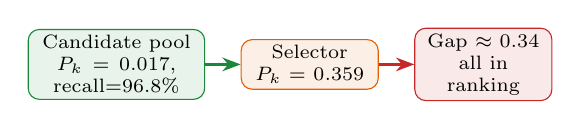
\begin{tikzpicture}[every node/.style={font=\scriptsize},arr/.style={-Stealth,thick},node distance=0.45cm]
\node[draw=green,fill=green!10,rounded corners,inner sep=2pt,text width=2.1cm,align=center] (cp)
  {Candidate pool\\ $P_k=0.017$, recall=96.8\%};
\node[draw=amber,fill=amber!10,rounded corners,inner sep=2pt,right=0.45cm of cp,text width=1.6cm,align=center] (sl)
  {Selector\\ $P_k=0.359$};
\node[draw=red,fill=red!10,rounded corners,inner sep=2pt,right=0.45cm of sl,text width=1.6cm,align=center] (gap)
  {Gap $\approx0.34$\\ all in ranking};
\draw[arr,green] (cp)--(sl); \draw[arr,red] (sl)--(gap);
\end{tikzpicture}
}\\[1pt]
Nearly perfect boundaries exist in the pool --- we cannot always pick them.
\textbf{Next step:} supervised boundary ranker ($\sim$50--100 labelled lectures).
}}

\medskip
\colorbox{red!10}{\parbox{\linewidth}{
\textcolor{red}{\textbf{Finding 2 — Granularity mismatch (most transferable result)}}\\[1pt]
{\footnotesize
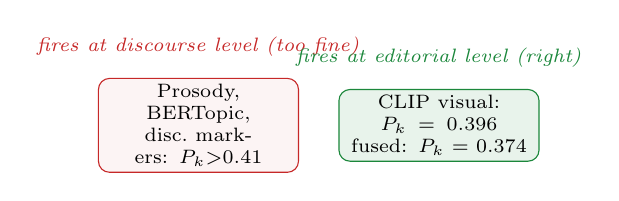
\begin{tikzpicture}[every node/.style={font=\scriptsize},node distance=0.35cm]
\node[draw=red,fill=red!5,rounded corners,inner sep=2pt,text width=2.4cm,align=center] (bad)
  {Prosody, BERTopic,\\ disc.\ markers: $P_k{>}0.41$};
\node[above=0.15cm of bad,font=\scriptsize,text=red] {\textit{fires at discourse level (too fine)}};
\node[draw=green,fill=green!10,rounded corners,inner sep=2pt,right=0.5cm of bad,text width=2.4cm,align=center] (good)
  {CLIP visual: $P_k=0.396$\\ fused: $P_k=0.374$};
\node[above=0.15cm of good,font=\scriptsize,text=green] {\textit{fires at editorial level (right)}};
\end{tikzpicture}
}\\[1pt]
Acoustic signals are accurate at the \textit{wrong} granularity.
CLIP succeeds because slide transitions are themselves editorial decisions.
}}

\hd{Statistical Evidence}
{\footnotesize Cross-model vs baseline: $P_k$, WD \textcolor{green}{\textbf{significant}} ($p<0.05$, Wilcoxon+Holm).
Selector vs cross-model: BS, F1 \textcolor{green}{\textbf{significant}}; $P_k$/WD \textcolor{amber}{\textbf{not significant}}.
Leave-domain-out: $P_k=0.4012$ (selector is a local operating point, not universal).}

\end{multicols}

\vspace{-6pt}
\colorbox{navy}{\parbox{\linewidth}{\vspace{3pt}\centering\small
\textcolor{white}{\textbf{Core claim:} LecSeg-30 does not solve lecture segmentation --- it makes it \textbf{measurable}, \textbf{inspectable}, and \textbf{reproducible}.}
\vspace{3pt}}}
\end{document}
